% ============================================================
%  3. DATA
% ============================================================
\chapter{Data}\label{sec:data}
 
All four series are retrieved from FRED (Federal Reserve Bank of St.\ Louis)
and share consistent, harmonised definitions across Denmark and the Eurozone.
 
\begin{table}[h!]
\centering
\begin{tabular}{llll}
\toprule
\textbf{Series} & \textbf{Region} & \textbf{FRED code} & \textbf{Definition} \\
\midrule
Unemployment rate & Denmark   & \texttt{LRHUADTTDKM156N}   & OECD harmonised, 25+, monthly \\
Unemployment rate & Euro area & \texttt{LRHUADTTEZM156N}   & OECD harmonised, 25+, monthly \\
HICP              & Denmark   & \texttt{CP0000DKM086NEST}  & Eurostat harmonised, not seas.\ adj., monthly \\
HICP              & Euro area & \texttt{CP0000EZ19M086NEST}& Eurostat harmonised, not seas.\ adj., monthly \\
\bottomrule
\end{tabular}
\caption{Data sources. Both unemployment series use identical OECD methodology
and the same 25+ age bracket, ensuring cross-country comparability.
Both HICP series are constructed under the same Eurostat rules,
making the inflation measures directly comparable.}
\end{table}

Since the Phillips curve concerns inflation rather than the price level, the HICP indices are transformed into year-on-year inflation rates. Inflation is computed as

\[
\pi_t = 100 \times \left(\frac{HICP_t}{HICP_{t-12}} - 1\right),
\]

where \(HICP_t\) denotes the harmonised consumer price index in month \(t\). Unemployment is kept in levels, as it is already measured as a rate.



\subsection{Inspections of raw data}
\subsubsection{Looking for trend}
We do find evidence for trend in both employments rate plots and for both inflation plots. Though the danish inflation seems very slight upward. There is a general large spike around COVID-19 period. Danish and Eurozone unemployment rate are relatively similar. Whereas when we look at the inflation, there is more low to not trend on the danish inflation level, where as there is a more clear upward trend for the Eurozone inflation.


\begin{figure}[H]
    \centering
    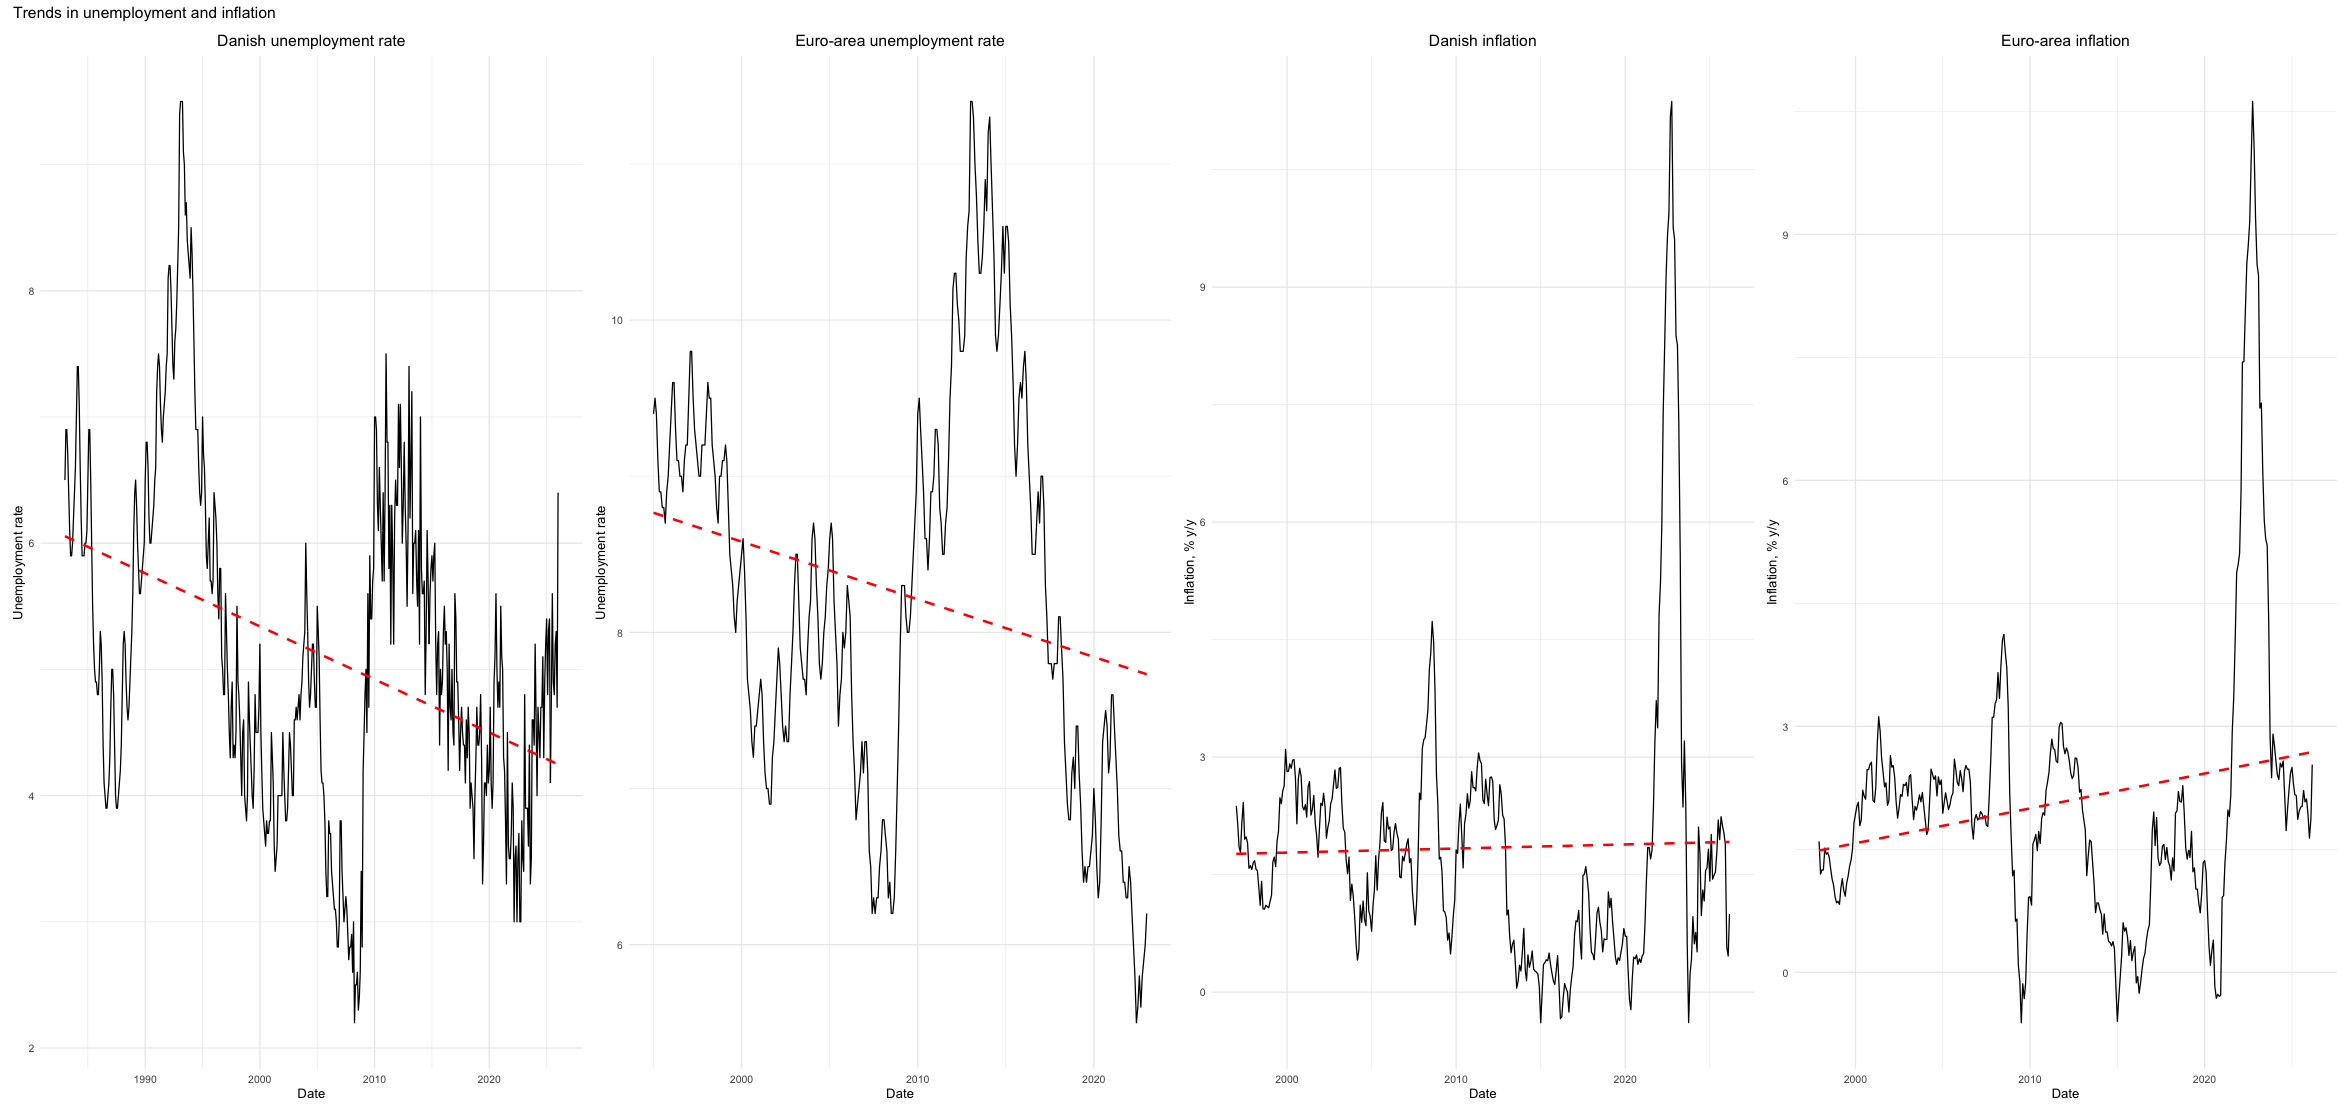
\includegraphics[width=1\linewidth]{billeder/raw_data_plot_trend.png}
    \caption{Both employment plots show a negative trend, and the inflations trends have a clear upward going trend}
    \label{fig:raw_data_plot_trend}
\end{figure}



\subsubsection{Looking for seasonality}


% ==== Bare lidt forklaring af dem hver  ======
% For Danish unemployment, there appears to be a mild seasonal pattern. Unemployment is often higher in the winter and early spring months, then tends to fall toward the summer, especially around June–August. However, the lines are quite noisy, so the seasonal pattern is not perfectly consistent across years.

% For Euro-area unemployment, the seasonal pattern is clearer. Many yearly lines decline from January/February toward the summer months and then rise again toward the end of the year. This suggests unemployment is typically lower in summer and higher in winter.

% For Danish inflation, there is no strong common seasonal pattern across years. Most yearly lines are clustered around relatively low inflation rates, while the years around COVID-19 show much higher inflation and dominate the plot. These outlier years reflect the unusual macroeconomic period rather than regular seasonality.

% For Euro-area inflation, the same applies. There is some variation across months, but the pattern is not stable across years. A few high-inflation years create visible spikes, especially later in the year, but this should not be interpreted as normal seasonal behavior



\begin{figure}[H]
    \centering
    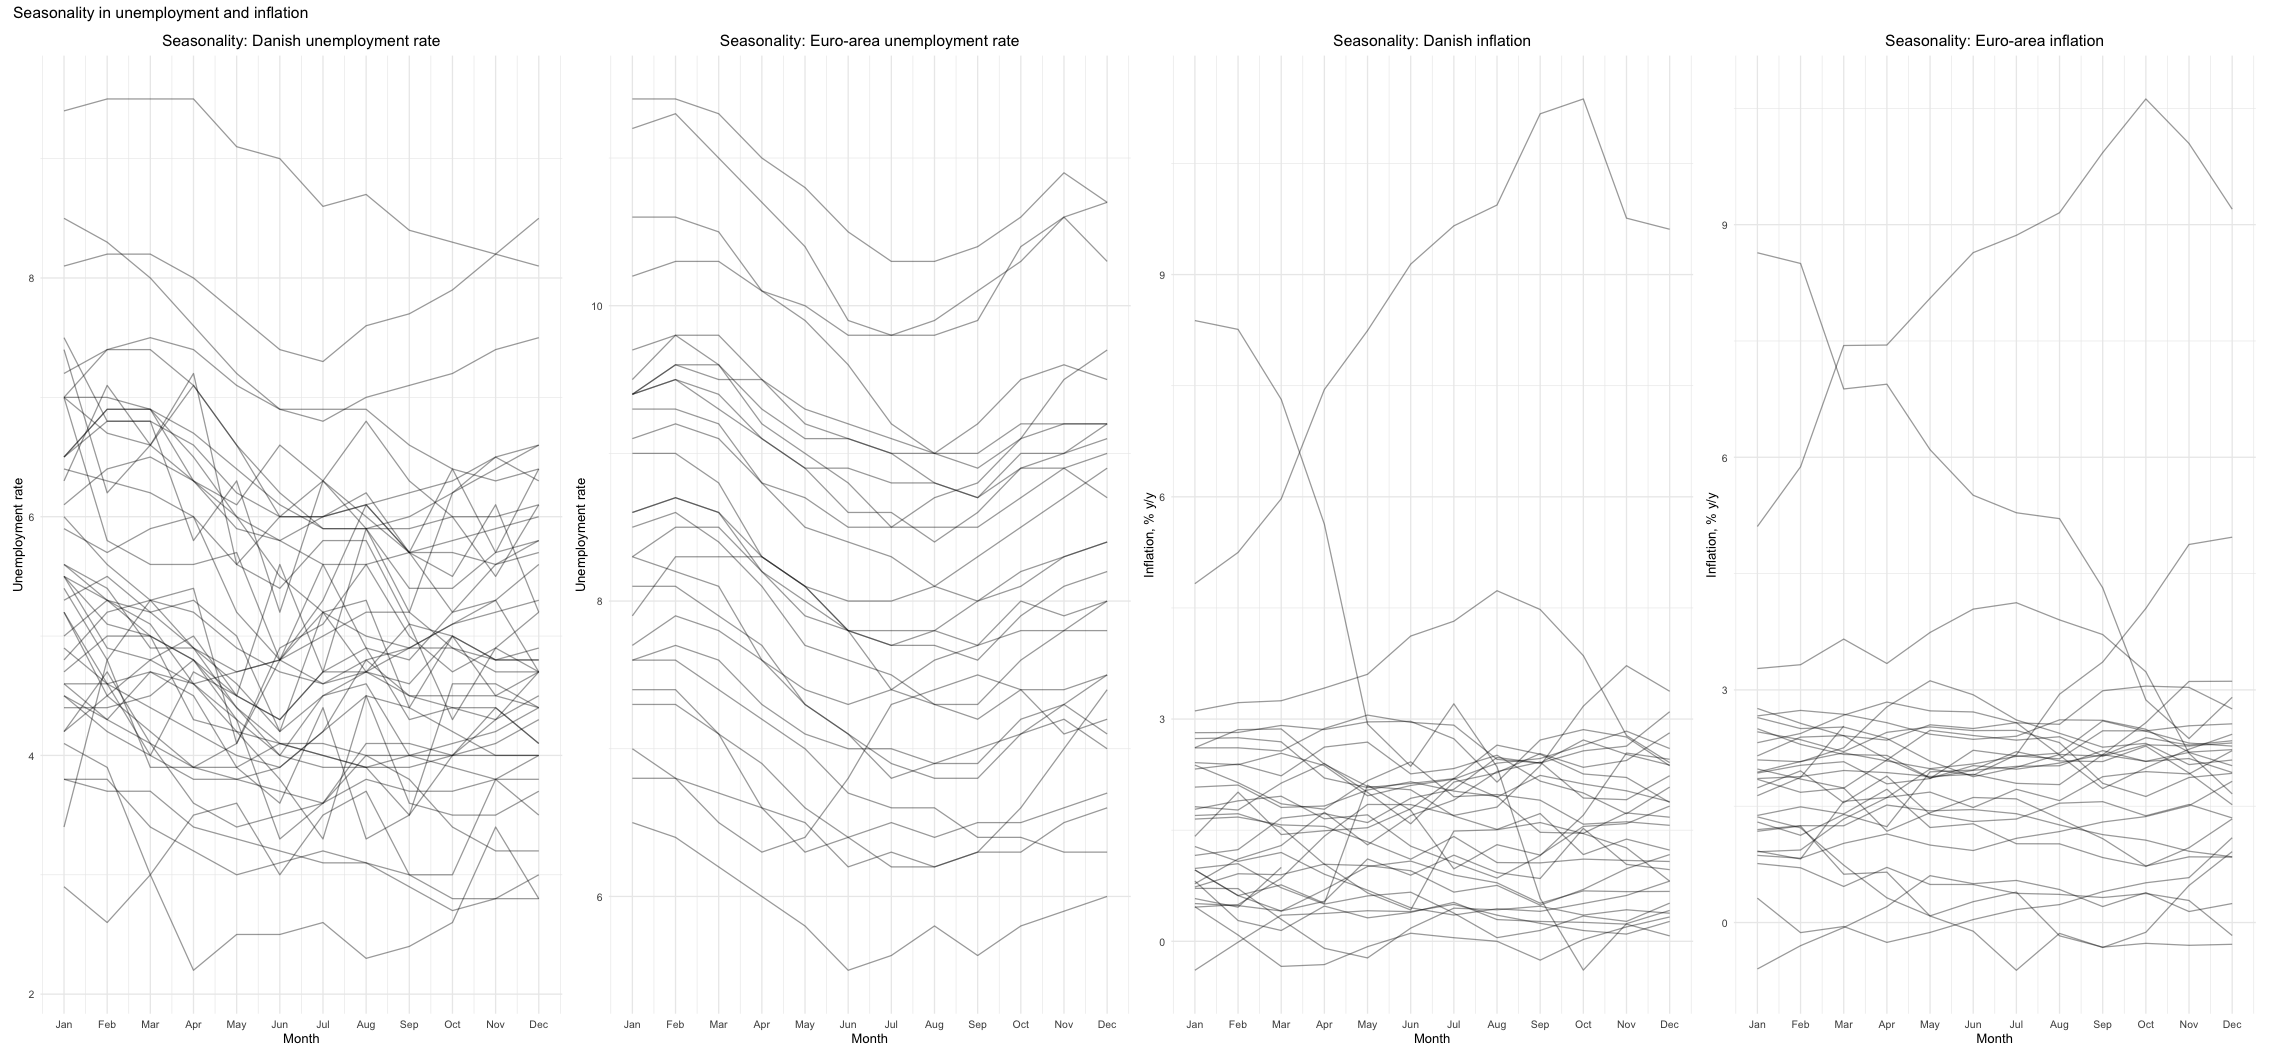
\includegraphics[width=1\linewidth]{billeder/indexed_seasonality_plot.png}
    \caption{Unemployment shows some seasonal behavior, especially in the euro area, while HICP shows little clear seasonality in this plot.}
    \label{fig:index_seasonal_plot}
\end{figure}


The seasonal plots indicate some recurring seasonal variation in unemployment, particularly for the euro area, where unemployment tends to be higher in winter and lower during the summer months. The pattern is weaker for Danish unemployment. In contrast, inflation displays less systematic seasonality. The inflation plots are dominated by a few high-inflation years, suggesting that variation is driven more by macroeconomic shocks than by stable monthly seasonal patterns.



% ==== subseries seasonal plot 

To examine this pattern more clearly, we next consider seasonal subseries plots, which compare observations within each calendar month over time. These plots confirm that unemployment contains a modest seasonal component, while inflation displays little evidence of stable seasonality. The inflation series are instead dominated by specific high-inflation episodes rather than regular monthly movements.

\begin{figure}[H]
    \centering
    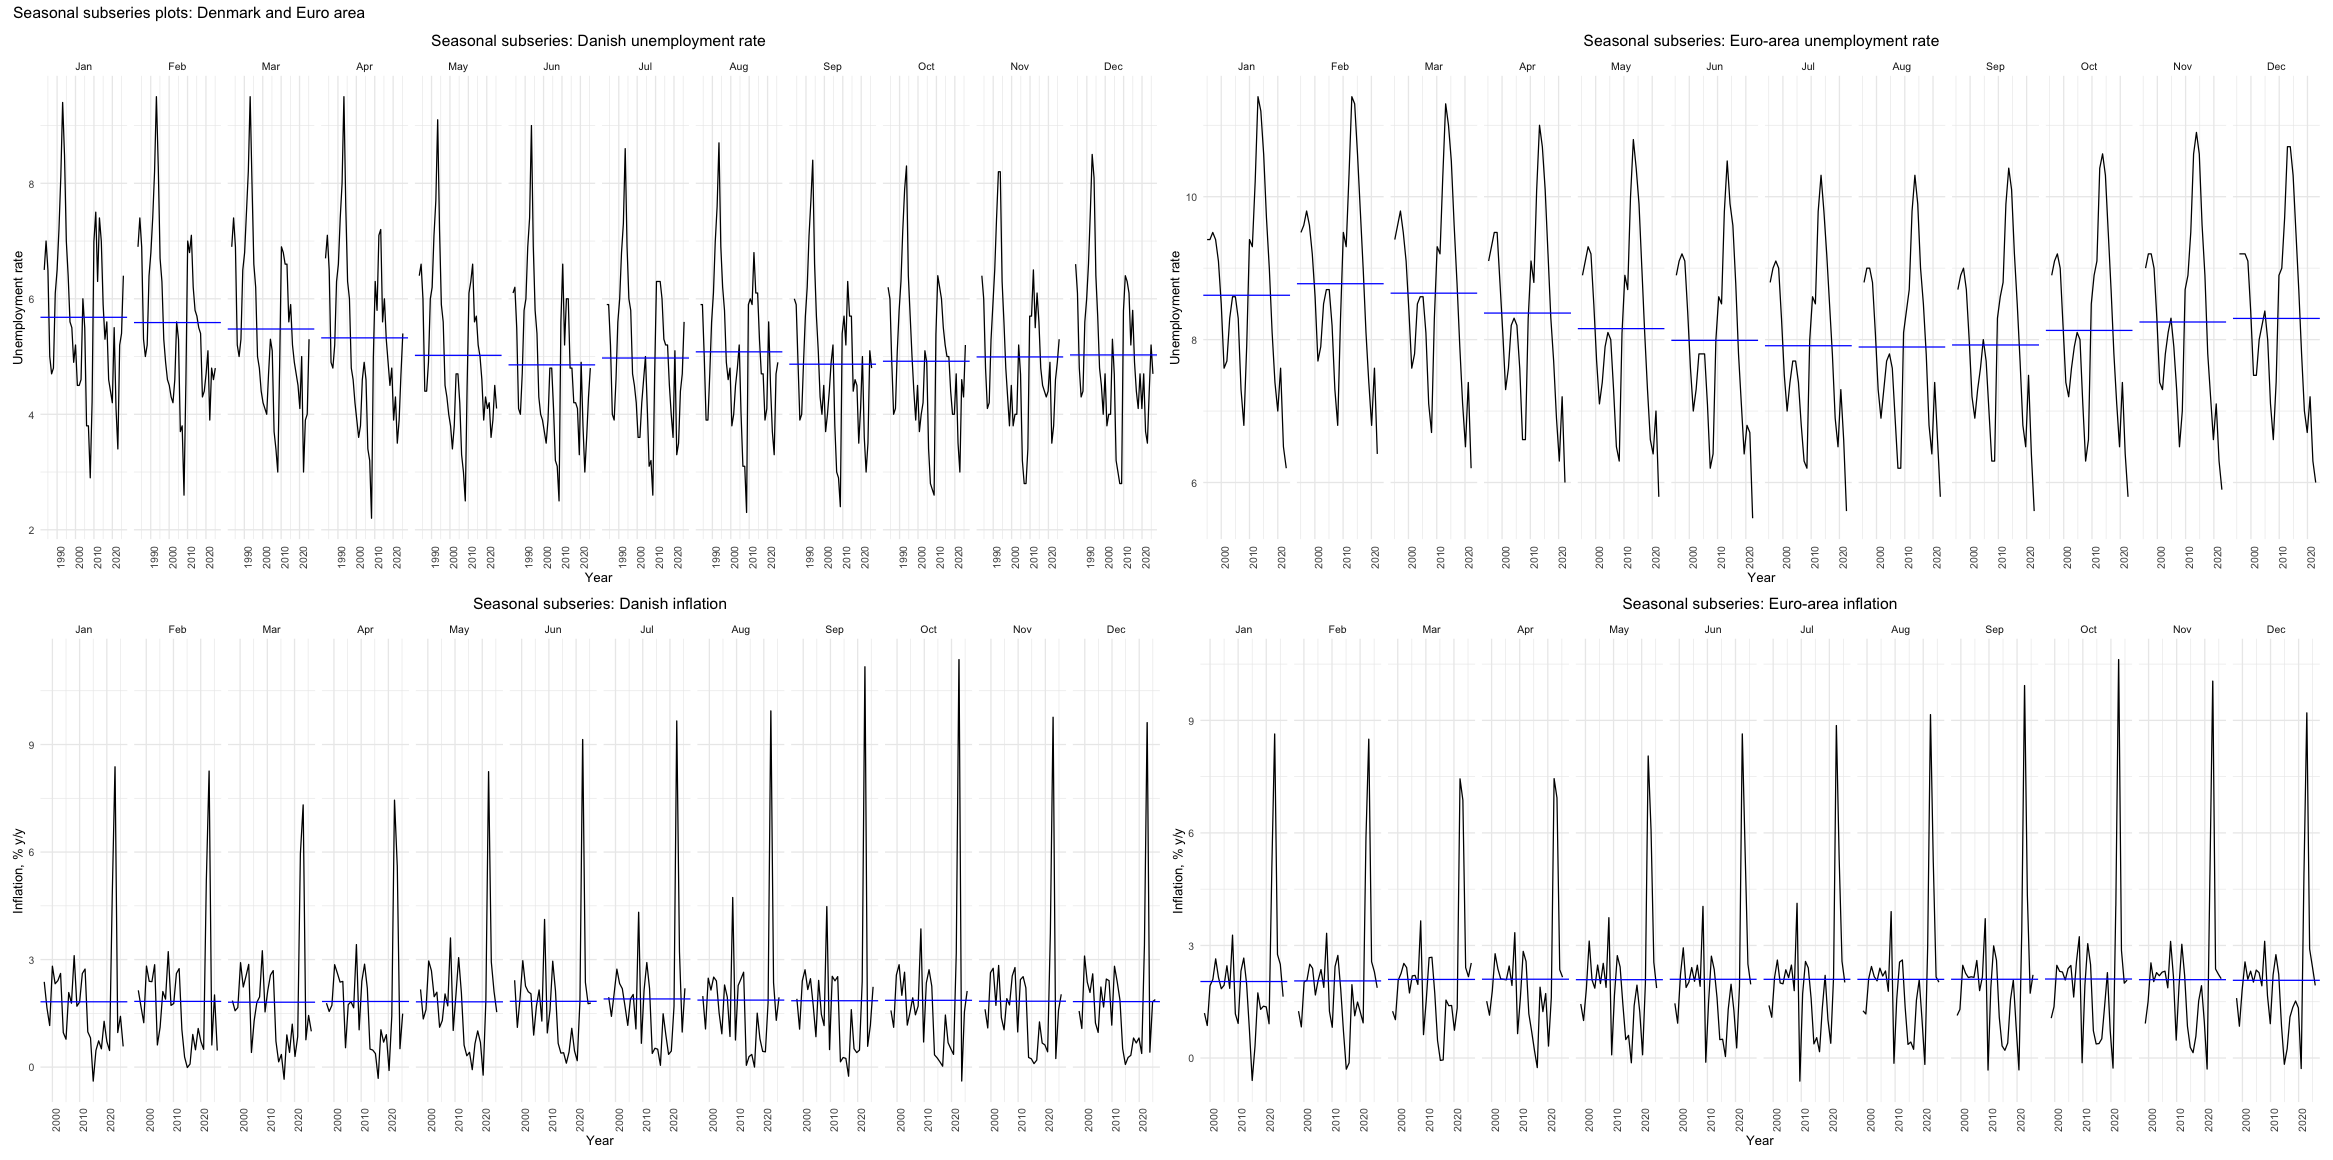
\includegraphics[width=1\linewidth]{billeder/seasonal_subseries_plot.png}
    \caption{The plots confirm that unemployment contains a modest seasonal component, while inflation displays little evidence of stable seasonality}
    \label{fig:seasonal_subseries_plot}
\end{figure}






\subsubsection{Testing for stationarity}

Before estimating the forecasting models, we assess stationarity using both the Augmented Dickey-Fuller (ADF) test and the KPSS test. The ADF test has non-stationarity as the null hypothesis, while the KPSS test has stationarity as the null hypothesis. Since the HICP indices have already been transformed into year-on-year inflation rates, the inflation variables are tested in growth-rate form.

\begin{table}[H]
\centering
\caption{Stationarity tests in levels}
\begin{tabular}{lcccc}
\hline
Variable & ADF p-value & ADF conclusion & KPSS p-value & KPSS conclusion \\
\hline
Danish unemployment & 0.7156 & Non-stationary & 0.0238 & Non-stationary \\
Euro-area unemployment & 0.9587 & Non-stationary & 0.0227 & Non-stationary \\
Danish inflation & 0.0996 & Weak evidence of stationarity & $>0.10$ & Stationary \\
Euro-area inflation & 0.2812 & Non-stationary & $>0.10$ & Stationary \\
\hline
\end{tabular}
\label{tab:stationarity_levels}
\end{table}

The results indicate that both unemployment variables are non-stationary in levels, as the ADF tests fail to reject non-stationarity and the KPSS tests reject stationarity. For inflation, the evidence is more mixed: the KPSS tests do not reject stationarity, while the ADF tests provide weaker evidence. Overall, unemployment appears clearly non-stationary, whereas inflation is more consistent with stationarity in levels.



\subsubsection{Plotting ACF for staitonarity}
The ACF plots support the findings from the stationarity tests. Both unemployment series display slowly declining autocorrelations that remain significant across many lags, indicating strong persistence and suggesting non-stationarity in levels. The inflation series are also persistent, but their autocorrelations decline more clearly toward zero. This is consistent with the mixed stationarity test results for inflation, where the evidence for non-stationarity is weaker than for unemployment.

\begin{figure}[H]
    \centering
    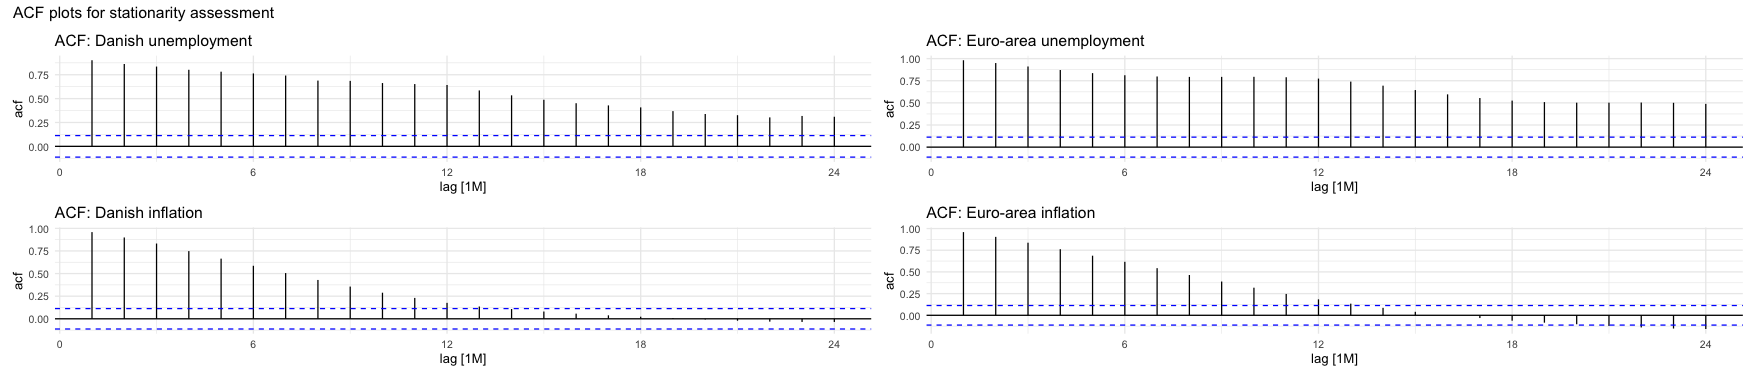
\includegraphics[width=1\linewidth]{billeder/ACF_plots_for_stationarity_assessment.png}
    \caption{Enter Caption}
    \label{fig:ACF_plots_for_stationarity_assessment}
\end{figure}



\subsubsection{Making the data stationary}

Since the level variables show evidence of non-stationarity, the variables are transformed using first differences:

\[
\Delta y_t = y_t - y_{t-1}.
\]

First differencing is chosen because it provides clear evidence of stationarity across all four variables. Seasonal differencing was also considered due to indications of annual dependence in the seasonal plots and ACFs, but it did not stationarize the series as clearly as first differencing. Any remaining seasonal dynamics are therefore handled in the modelling stage rather than by applying seasonal differencing mechanically to all variables.

\begin{table}[H]
\centering
\caption{Stationarity tests after first differencing}
\begin{tabular}{lccc}
\hline
Variable & ADF p-value & KPSS p-value & Conclusion \\
\hline
Danish unemployment & $<0.01$ & $>0.10$ & Stationary \\
Euro-area unemployment & $<0.01$ & $>0.10$ & Stationary \\
Danish inflation & $<0.01$ & $>0.10$ & Stationary \\
Euro-area inflation & 0.0114 & $>0.10$ & Stationary \\
\hline
\end{tabular}
\label{tab:stationarity_first_diff}
\end{table}

The tests confirm that the first-differenced variables are stationary: the ADF tests reject non-stationarity, while the KPSS tests fail to reject stationarity. The ACF plots in Figure~\ref{fig:difference_ACF_plot} support this conclusion, as the slow decay observed in levels is largely removed. Some seasonal autocorrelation remains, especially for euro-area unemployment around lags 12 and 24, suggesting that seasonal dynamics may still be relevant in the forecasting models.

\begin{figure}[H]
    \centering
    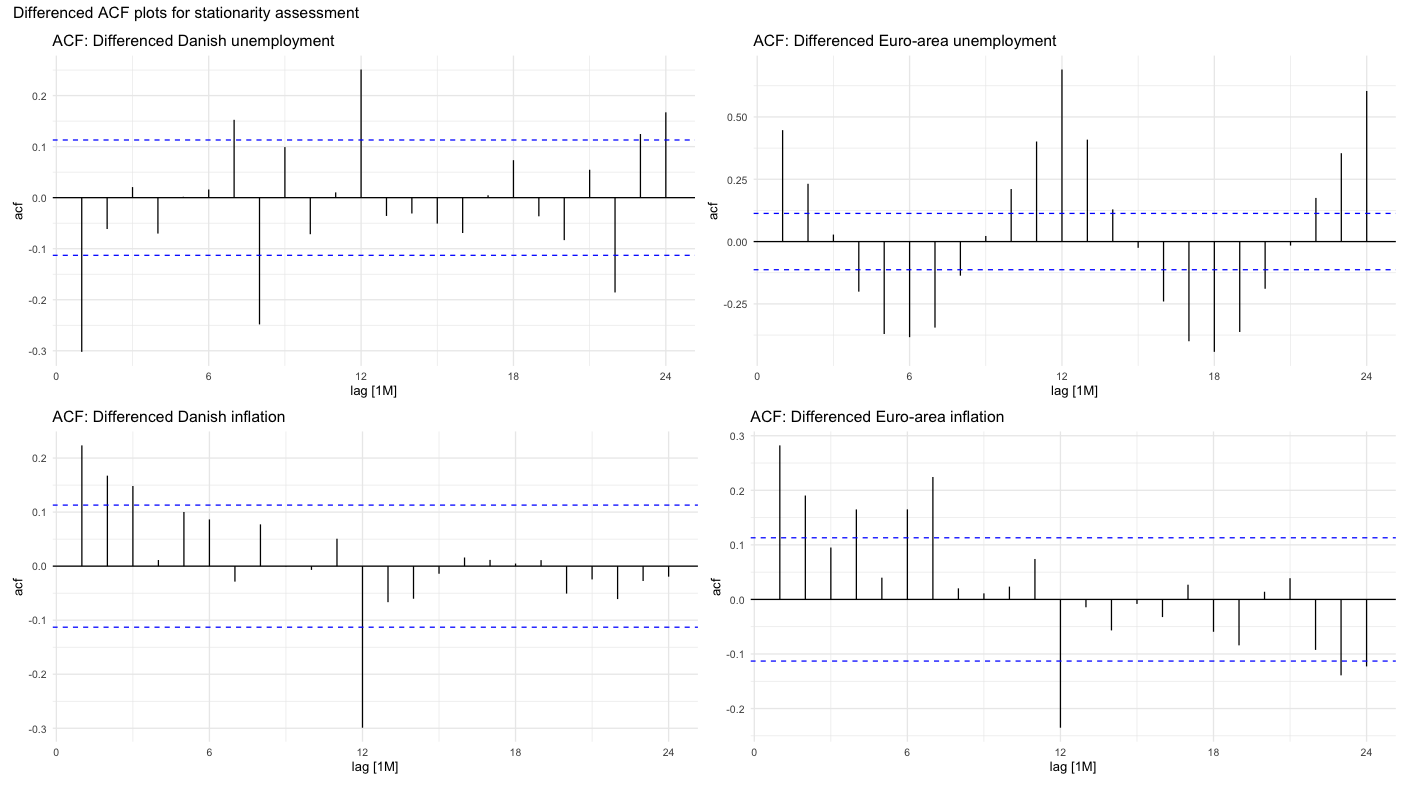
\includegraphics[width=1\linewidth]{billeder/difference_ACF_plot.png}
    \caption{ACF plots of the first-differenced variables}
    \label{fig:difference_ACF_plot}
\end{figure}


\subsection{Fitting the Arima}

The univariate ARIMA model serves as the benchmark model. Its purpose is to assess how well Danish inflation can be forecast using only its own past values. Since the stationarity tests indicate that Danish inflation is stationary after first differencing, the ARIMA benchmark is estimated on first-differenced Danish inflation:
\[
\Delta \pi_t^{DK} = \pi_t^{DK} - \pi_{t-1}^{DK}.
\]


The ARIMA benchmark selected for first-differenced Danish inflation is
\[
ARIMA(1,0,1)(0,0,1)_{12}.
\]
The presence of a seasonal moving-average term indicates remaining annual dependence in Danish inflation, which is consistent with the ACF/PACF evidence around lag 12. Thus, seasonality is handled within the ARIMA specification rather than through additional seasonal differencing. The model obtains an AIC of 144.51, an AICc of 144.64, and a BIC of 159.34, which provide the benchmark values for later model comparison. \textcolor{red}{Lidt usikker på hvordan vi bedst lige håndterer den mini seasonalit der er. Men sådan her er jeg endt med at gøre det}

The residual diagnostics indicate that the ARIMA benchmark is adequate. The residual ACF shows no clear remaining autocorrelation, and the Ljung-Box test fails to reject the null of no residual autocorrelation at lag 24, with \(p = 0.3869\). Hence, the model appears to capture the main serial dependence in first-differenced Danish inflation. Some outliers remain, likely reflecting the exceptional post-COVID inflation period.

\begin{figure}
    \centering
    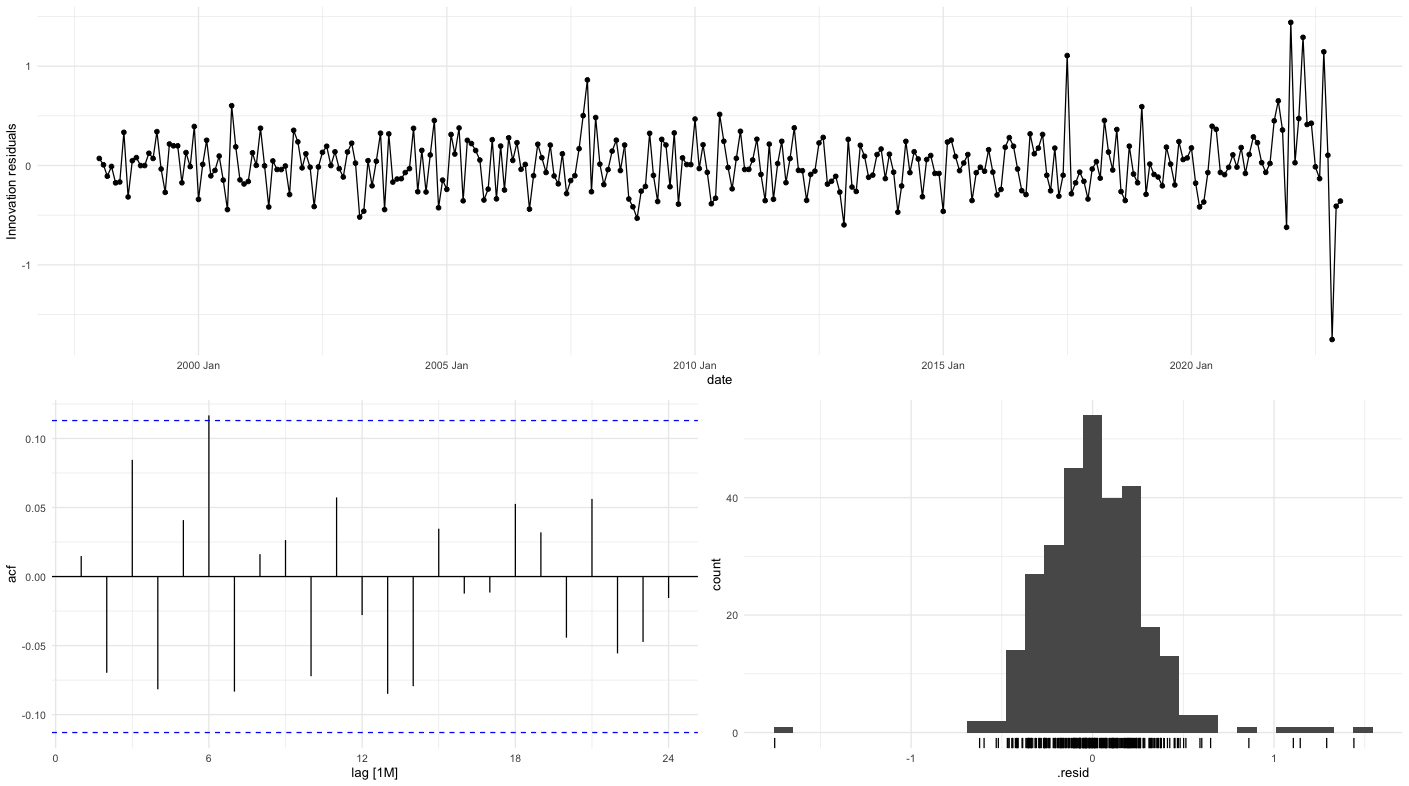
\includegraphics[width=0.5\linewidth]{billeder/plot_residuals_ARIMA_benchmark.png}
    \caption{Enter Caption}
    \label{fig:placeholder}
\end{figure}








